\section{Results} \label{sec:results}

Using the dataset described in the previous section, we replicated the experiments in \cite{ssk} that evaluated the effect of changing the length parameter of the SSK and NGK kernels. The results of our experiments can be seen in Figure \ref{fig:ours} with the results of the original paper shown in Figure \ref{fig:theirs} for contrast. For specific results regarding each seperate category, please see the tables located in the \texttt{results} directory on the Git repository \cite{git}.

From the plots of the average F1 score over all categories, we show that we were able to achieve comparable results for length parameter values up to 7. For higher values the classification results seem to deteriorate for both NGK and SSK. Upon further inspection we found that the classification for categories \textit{crude} and \textit{corn}, which have the lowest number of test and training documents, are affected the most.

\begin{figure}[H]
  \centering
  \begin{subfigure}{0.5\textwidth}
    \centering
    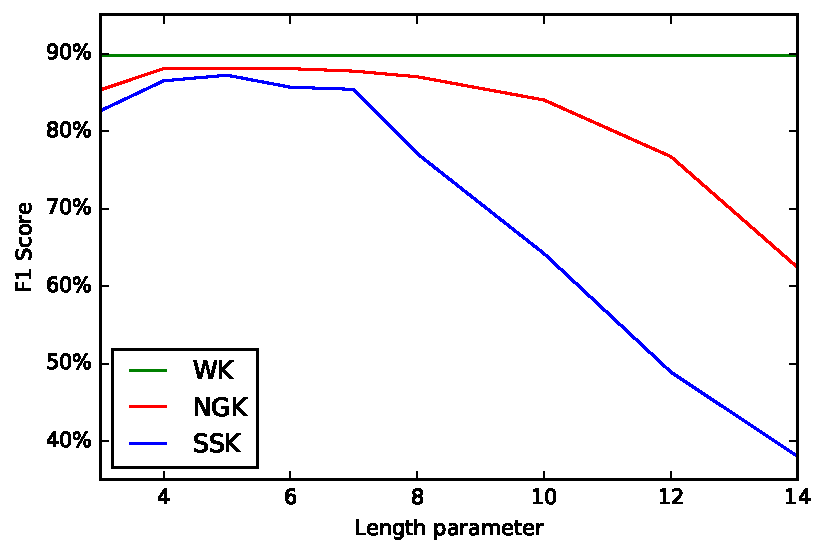
\includegraphics[width=1.0\linewidth]{figures/ours.pdf}
    \caption{Our results}
    \label{fig:ours}
  \end{subfigure}%
  \begin{subfigure}{0.5\textwidth}
    \centering
    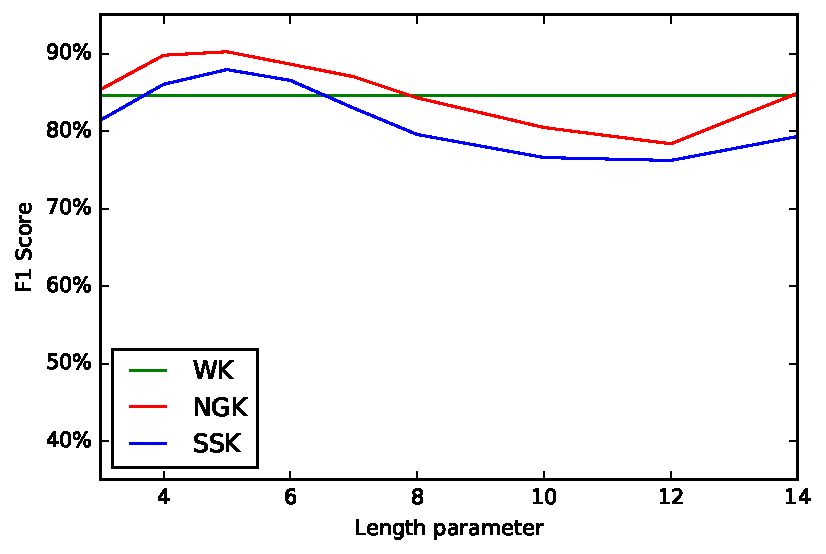
\includegraphics[width=1.0\linewidth]{figures/theirs.pdf}
    \caption{Results from original paper}
    \label{fig:theirs}
  \end{subfigure}
  \caption{Mean F1 score with different length parameters for the WK, NGK, and SSK kernels. The mean is computed over the categories \textit{acq}, \textit{corn}, \textit{crude}, and \textit{earn}.}
  \label{fig:oursvstheirs}
\end{figure}
